\documentclass[11pt,a4paper]{article}

% ---------------------------------------------------------------------------
% GitFlame CodeRAG -- final project report.
% Structure, tables and figure placeholders prepared by Kirill.
% Tables under reports/tables/ are auto-generated by scripts/build_latex_tables.py.
% ---------------------------------------------------------------------------

\usepackage[margin=2.5cm]{geometry}
\usepackage[T1]{fontenc}
\usepackage[utf8]{inputenc}
\usepackage{amsmath,amssymb}
\usepackage{booktabs}
\usepackage{graphicx}
\usepackage{xcolor}
\usepackage{caption}
\usepackage{enumitem}
\usepackage{tikz}
\usetikzlibrary{arrows.meta,positioning}
\usepackage[hidelinks]{hyperref}

% Placeholder helpers (for results produced later in the project).
\newcommand{\placeholder}[1]{{\color{gray}\itshape [#1]}}
\newcommand{\figplaceholder}[2]{%
  \IfFileExists{figures/#1}{\includegraphics[width=\linewidth]{figures/#1}}{%
    \fbox{\parbox[c][3.2cm][c]{0.98\linewidth}{\centering\color{gray}\itshape
      Placeholder for \texttt{\detokenize{figures/#1}}\\[2pt]#2}}}%
}

\title{\textbf{GitFlame CodeRAG}\\[2pt]
  Hybrid Issue-to-Evidence Retrieval for Repository Workflows\\[4pt]
  \large Final Project Report: From Repository Ingestion to Ranked Evidence}
\author{GitFlame CodeRAG Team\\
  Danil, Karim, Evgeny, Martin, Kirill}
\date{\today}

\begin{document}
\maketitle

\begin{abstract}
GitFlame CodeRAG retrieves relevant code evidence for a GitHub/GitFlame-like issue,
producing top-$k$ evidence chunks (with file paths, line ranges, metadata and scores)
suitable for downstream plan and code generation. This report describes the
complete project, from dataset construction and repository ingestion to the full
end-to-end retrieval pipeline and its evaluation. The pipeline an issue is expanded into keywords and symbols, three retrievers
(lexical BM25, dense code embeddings, and AST-structural candidates) generate
candidates, their rankings are fused with Reciprocal Rank Fusion (RRF), and a
cross-encoder reranker produces the final ranking. We evaluate the pipeline on a
curated, tiered dataset of 22 synthetic repositories (about 1.25M code chunks) with known
\emph{expected files}, using Recall@K, MRR and MAP/NDCG, and quantify the
contribution of each component through ablations and statistical significance
tests. This report presents the dataset, method, experimental protocol and
reproducibility setup; result tables and figures are wired to the evaluation
outputs and are filled automatically as experiments complete.
\end{abstract}

\section{Introduction}
The GitFlame CodePilot assistant helps developers act on repository issues. This
project focuses on the retrieval/RAG component for the \emph{issue-to-plan} and
later \emph{plan-to-code} scenarios: given repository code files, a repository
\texttt{.yml} configuration and an issue, return the top-$k$ code chunks that
constitute the best evidence for resolving the issue. Recommendations and full
code generation are out of scope; the target is \emph{issue $\rightarrow$ relevant
code evidence}. The central design principle is that raw source code is preserved
as the source of truth (line numbers, real syntax), while separate normalized
representations are used only for search (BM25 text, embedding text, keywords).

\section{Related Work}
Our pipeline combines three complementary retrieval signals. \emph{Lexical}
retrieval with BM25 ranks chunks by term overlap and remains a strong baseline for
code search. \emph{Dense} retrieval embeds queries and code chunks into a shared
vector space with a code-aware embedding model and ranks by cosine similarity,
capturing semantic matches that lexical methods miss. \emph{Structural} retrieval
uses AST-Grep to extract functions, handlers, tests and configuration nodes and to
find candidates by symbols and structural patterns; it complements natural-language
retrieval rather than replacing it. To combine rankers we use Reciprocal Rank
Fusion, a simple and robust rank-aggregation method, followed by a cross-encoder
\emph{reranker} that jointly scores each query--chunk pair for a final ordering.

\section{Dataset}
\label{sec:dataset}
The evaluation dataset is organised into three size tiers so that retrieval and
indexing can be exercised from small, human-readable repositories up to
codebase-scale inputs. The \emph{small} tier contains 15 curated multi-language
repositories with realistic source files (functions, classes, handlers, imports);
the \emph{medium} tier adds 5 synthetic repositories of 50{,}000 chunks each; and
the \emph{large} tier adds 2 repositories of 500{,}000 chunks each, for roughly
1.25M code chunks in total. Every repository ships a \texttt{repo.yml} configuration
and seven GitHub-like issues; each issue provides \texttt{id}, \texttt{title},
\texttt{body}, \texttt{labels} and \texttt{expected\_files} (the ground-truth
retrieval labels), while \texttt{expected\_chunks} are intentionally out of scope.
Under the default \texttt{ast\_aware} chunking each top-level definition becomes one
chunk, so the synthetic tiers are sized directly in chunk units. Table~\ref{tab:datagroups}
summarises every repository grouped by tier.

\begin{table}[h]
\centering
\caption{Dataset overview across the three size tiers: files, chunks,
issues and expected-file labels per repository, with per-tier subtotals and grand total.}
\label{tab:datagroups}
\footnotesize
% Auto-generated by scripts/build_dataset_table.py -- do not edit by hand.
\begin{tabular}{l r r r r}
\toprule
Repository & Files & Chunks & Issues & Exp.\ labels \\
\midrule
\multicolumn{5}{l}{\textbf{Small ($<$50k chunks)} -- 15 repositories} \\
\midrule
\texttt{repo\_001\_fastapi\_blog} & 8 & 23 & 7 & 12 \\
\texttt{repo\_002\_go\_url\_shortener} & 6 & 14 & 7 & 10 \\
\texttt{repo\_003\_express\_todo\_api} & 6 & 11 & 7 & 11 \\
\texttt{repo\_004\_react\_dashboard} & 6 & 13 & 7 & 11 \\
\texttt{repo\_005\_flask\_auth\_service} & 6 & 16 & 7 & 11 \\
\texttt{repo\_006\_go\_grpc\_inventory} & 6 & 17 & 7 & 12 \\
\texttt{repo\_007\_django\_shop} & 7 & 13 & 7 & 11 \\
\texttt{repo\_008\_vue\_notes\_app} & 6 & 10 & 7 & 10 \\
\texttt{repo\_009\_nestjs\_payments} & 6 & 8 & 7 & 10 \\
\texttt{repo\_010\_rust\_cli\_tool} & 5 & 8 & 7 & 11 \\
\texttt{repo\_011\_python\_etl\_pipeline} & 6 & 9 & 7 & 9 \\
\texttt{repo\_012\_node\_ts\_graphql} & 6 & 12 & 7 & 12 \\
\texttt{repo\_013\_python\_lru\_cache} & 4 & 13 & 7 & 9 \\
\texttt{repo\_014\_python\_task\_queue} & 4 & 11 & 7 & 8 \\
\texttt{repo\_015\_python\_state\_machine} & 4 & 11 & 7 & 10 \\
\multicolumn{1}{r}{\emph{subtotal}} & 86 & 189 & 105 & 157 \\
\midrule
\multicolumn{5}{l}{\textbf{Medium (50k chunks)} -- 5 repositories} \\
\midrule
\texttt{repo\_medium\_001} & 100 & 50000 & 7 & 7 \\
\texttt{repo\_medium\_002} & 100 & 50000 & 7 & 7 \\
\texttt{repo\_medium\_003} & 100 & 50000 & 7 & 7 \\
\texttt{repo\_medium\_004} & 100 & 50000 & 7 & 7 \\
\texttt{repo\_medium\_005} & 100 & 50000 & 7 & 7 \\
\multicolumn{1}{r}{\emph{subtotal}} & 500 & 250000 & 35 & 35 \\
\midrule
\multicolumn{5}{l}{\textbf{Large (500k chunks)} -- 2 repositories} \\
\midrule
\texttt{repo\_large\_001} & 1000 & 500000 & 7 & 7 \\
\texttt{repo\_large\_002} & 1000 & 500000 & 7 & 7 \\
\multicolumn{1}{r}{\emph{subtotal}} & 2000 & 1000000 & 14 & 14 \\
\midrule
\textbf{Total} & \textbf{2586} & \textbf{1250189} & \textbf{154} & \textbf{206} \\
\bottomrule
\end{tabular}

\end{table}

\begin{table}[h]
\centering
\caption{Language distribution of the small tier.}
\label{tab:langs}
% Auto-generated by scripts/build_latex_tables.py -- do not edit by hand.
\begin{tabular}{l r}
\toprule
Language & Repositories \\
\midrule
go & 2 \\
javascript & 3 \\
python & 4 \\
rust & 1 \\
typescript & 4 \\
\bottomrule
\end{tabular}

\end{table}

\section{Method}
\label{sec:method}
The end-to-end pipeline transforms an issue into ranked evidence chunks
(Figure~\ref{fig:pipeline}). Repository files are loaded, filtered by the
\texttt{.yml} config and split into AST-aware chunks (with a fixed-window fallback);
each chunk carries structural metadata, a BM25 text, an embedding text and keywords, and chunks, metadata and embeddings are persisted (PostgreSQL/pgvector) for retrieval.
At query time the issue is converted into a query text and keywords, the three
retrievers produce candidate lists, RRF fuses them, and the reranker orders the
fused candidates into the final top-$k$.

\begin{figure}[h]
\centering
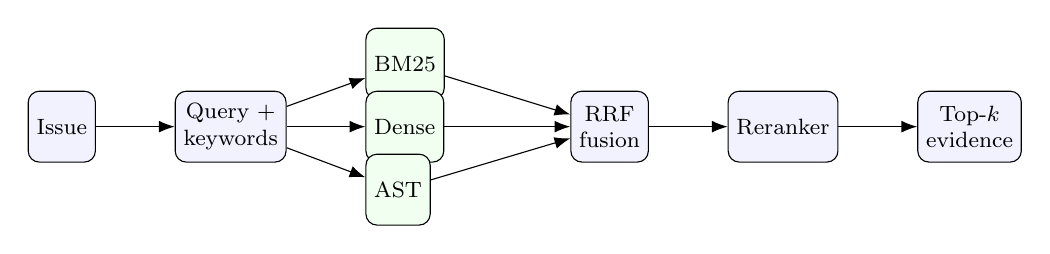
\begin{tikzpicture}[
  node distance=8mm and 10mm,
  box/.style={draw,rounded corners,align=center,minimum height=9mm,
    inner sep=3pt,font=\footnotesize,fill=blue!5},
  ret/.style={box,fill=green!6},
  arr/.style={-{Latex[length=2mm]}}]
  \node[box] (issue) {Issue};
  \node[box,right=of issue] (q) {Query +\\keywords};
  \node[ret,right=of q,yshift=8mm] (bm25) {BM25};
  \node[ret,right=of q] (dense) {Dense};
  \node[ret,right=of q,yshift=-8mm] (ast) {AST};
  \node[box,right=16mm of dense] (rrf) {RRF\\fusion};
  \node[box,right=of rrf] (rer) {Reranker};
  \node[box,right=of rer] (topk) {Top-$k$\\evidence};
  \draw[arr] (issue) -- (q);
  \draw[arr] (q) -- (bm25);
  \draw[arr] (q) -- (dense);
  \draw[arr] (q) -- (ast);
  \draw[arr] (bm25) -- (rrf);
  \draw[arr] (dense) -- (rrf);
  \draw[arr] (ast) -- (rrf);
  \draw[arr] (rrf) -- (rer);
  \draw[arr] (rer) -- (topk);
\end{tikzpicture}
\caption{End-to-end retrieval pipeline: issue $\rightarrow$ BM25 / Dense / AST
$\rightarrow$ RRF $\rightarrow$ reranker $\rightarrow$ final top-$k$ evidence chunks.}
\label{fig:pipeline}
\end{figure}

\paragraph{Dense similarity.} Query and chunk embeddings are compared with cosine
similarity,
\begin{equation}
\mathrm{sim}(q, c) = \frac{\mathbf{e}_q \cdot \mathbf{e}_c}
{\lVert \mathbf{e}_q \rVert \, \lVert \mathbf{e}_c \rVert}.
\end{equation}

\paragraph{Rank fusion.} Given rankings $R_1,\dots,R_m$ from the retrievers, RRF
scores each chunk $c$ by
\begin{equation}
\mathrm{RRF}(c) = \sum_{i=1}^{m} \frac{1}{k + \mathrm{rank}_i(c)},
\end{equation}
where $\mathrm{rank}_i(c)$ is the 1-based rank of $c$ in $R_i$ (absent chunks
contribute $0$) and $k$ is a smoothing constant (\texttt{rrf\_k}). The reranker then
assigns a joint relevance score to each surviving query--chunk pair, and the final
top-$k$ evidence chunks are emitted in the shared evidence format. When the reranker
model is unavailable, the pipeline falls back to the RRF ordering.

\section{Experimental Setup}
\label{sec:setup}
\paragraph{Ablations.} We evaluate each signal and their combination:
(i)~BM25 only, (ii)~Dense only, (iii)~AST candidates only, (iv)~RRF over all three,
and (v)~RRF~+~reranker. This isolates the contribution of lexical, semantic and
structural evidence and of the reranking stage.

\paragraph{Metrics.} Using \texttt{expected\_files} as ground truth we report
Recall@K, Mean Reciprocal Rank (MRR), Mean Average Precision (MAP) and NDCG@K for
$K \in \{1,3,5,10\}$, macro-averaged over the 84 issues.

\paragraph{Hyperparameters.} Table~\ref{tab:hparams} lists the search grid for the
per-retriever candidate depths, the RRF constant, and the reranker/final cut-offs.

\begin{table}[h]
\centering
\caption{Hyperparameter search grid.}
\label{tab:hparams}
% Auto-generated by scripts/build_latex_tables.py -- do not edit by hand.
\begin{tabular}{l l}
\toprule
Hyperparameter & Search values \\
\midrule
\texttt{bm25\_top\_k} & 50, 100 \\
\texttt{dense\_top\_k} & 50, 100 \\
\texttt{ast\_top\_k} & 20, 50 \\
\texttt{rrf\_k} & 60 \\
\texttt{reranker\_top\_k} & 20, 50 \\
\texttt{final\_top\_k} & 5, 10 \\
\bottomrule
\end{tabular}

\end{table}

\paragraph{Significance testing.} For the headline comparisons (e.g.\ RRF vs.\ each
single retriever, and RRF~+~reranker vs.\ RRF) we test per-issue metric differences
for significance and report the effect size and $p$-value.

\section{Results}
\label{sec:results}
Table~\ref{tab:ablation} reports the ablation metrics and Table~\ref{tab:sig} the
significance tests; numbers are populated from the evaluation outputs
(\texttt{reports/results/}). Figure~\ref{fig:recall} shows Recall@K curves per method.

\begin{table}[h]
\centering
\caption{Ablation results (macro-averaged over 84 issues). \placeholder{filled from
reports/results/metrics.json}}
\label{tab:ablation}
\small
% Auto-generated by scripts/build_latex_tables.py.
% Fill reports/results/metrics.json to replace placeholders with real numbers.
\begin{tabular}{lrrrrrr}
\toprule
Method & R@1 & R@5 & R@10 & MRR & MAP & NDCG@10 \\
\midrule
BM25 & \phantom{0.000}-- & \phantom{0.000}-- & \phantom{0.000}-- & \phantom{0.000}-- & \phantom{0.000}-- & \phantom{0.000}-- \\
Dense & \phantom{0.000}-- & \phantom{0.000}-- & \phantom{0.000}-- & \phantom{0.000}-- & \phantom{0.000}-- & \phantom{0.000}-- \\
AST candidates & \phantom{0.000}-- & \phantom{0.000}-- & \phantom{0.000}-- & \phantom{0.000}-- & \phantom{0.000}-- & \phantom{0.000}-- \\
RRF (BM25+Dense+AST) & \phantom{0.000}-- & \phantom{0.000}-- & \phantom{0.000}-- & \phantom{0.000}-- & \phantom{0.000}-- & \phantom{0.000}-- \\
RRF + Reranker & \phantom{0.000}-- & \phantom{0.000}-- & \phantom{0.000}-- & \phantom{0.000}-- & \phantom{0.000}-- & \phantom{0.000}-- \\
\bottomrule
\end{tabular}

\end{table}

\begin{figure}[h]
\centering
\figplaceholder{recall_at_k.pdf}{Recall@K curves per method will be inserted here.}
\caption{Recall@K per retrieval configuration.}
\label{fig:recall}
\end{figure}

\begin{table}[h]
\centering
\caption{Statistical significance of headline comparisons. \placeholder{filled from
reports/results/significance.json}}
\label{tab:sig}
% Auto-generated by scripts/build_latex_tables.py.
% Fill reports/results/significance.json to replace placeholders.
\begin{tabular}{l l r r}
\toprule
Comparison & Metric & $\Delta$ & $p$-value \\
\midrule
RRF vs BM25 & NDCG@10 & \phantom{0.000}-- & \phantom{0.000}-- \\
RRF vs Dense & NDCG@10 & \phantom{0.000}-- & \phantom{0.000}-- \\
RRF+Reranker vs RRF & NDCG@10 & \phantom{0.000}-- & \phantom{0.000}-- \\
\bottomrule
\end{tabular}

\end{table}

\placeholder{Discussion of which signals help which issue types, and whether the
reranker gain over RRF is significant, to be written once results are in.}

\section{Reproducibility}
\label{sec:repro}
Every experiment input is described by a single generated manifest,
\texttt{experiment\_manifest.yml}, listing per repository its config, code and issues
paths, revision, file and issue counts, and \texttt{expected\_files} coverage, plus the
experiment matrix and hyperparameter grid. The manifest is produced by
\texttt{scripts/build\_manifest.py} and validated by
\texttt{validate\_experiment\_inputs()}, which reuses the ingestion functions to
confirm that each \texttt{.yml} parses, code files load, issues are well-formed, and
every \texttt{expected\_file} exists and passes config filtering. On the current
small tier all 15 repositories validate with zero errors. Report tables are
regenerated from the manifest and results by \texttt{scripts/build\_latex\_tables.py},
so the document stays consistent with the data.

\section{Conclusion and Future Work}
The project delivers the full issue-to-evidence pipeline (repository ingestion and
indexing, then BM25/Dense/AST $\rightarrow$ RRF $\rightarrow$ reranker), a reproducible
experiment manifest and input validation, and a report wired to the evaluation outputs. Once the ablation and significance
runs complete, the result tables and figures populate automatically. Future work
includes richer issue-query construction, learned fusion weights, and extending the
dataset toward \texttt{expected\_chunks} for finer-grained evaluation.

\begin{thebibliography}{9}
\bibitem{bm25} S.~Robertson and H.~Zaragoza. \emph{The Probabilistic Relevance
Framework: BM25 and Beyond}. Foundations and Trends in Information Retrieval, 2009.
\bibitem{rrf} G.~V.~Cormack, C.~L.~A.~Clarke, and S.~Buettcher. \emph{Reciprocal Rank Fusion Outperforms Condorcet and Individual Rank Learning Methods}. SIGIR, 2009.
\bibitem{dpr} V.~Karpukhin et al. \emph{Dense Passage Retrieval for Open-Domain Question Answering}. EMNLP, 2020.
\end{thebibliography}

\end{document}
